\documentclass[12pt]{article}%
\usepackage{amsfonts}
\usepackage{fancyhdr}
\usepackage{comment}
\usepackage[colorlinks]{hyperref}
\usepackage{fancyvrb}
\usepackage{lipsum}
\usepackage[a4paper, top=2.5cm, bottom=2.5cm, left=2.2cm, right=2.2cm]%
{geometry}
\usepackage{times}
\usepackage{amsmath}
\usepackage{subfig}
\usepackage{changepage}
\usepackage{amssymb}
\usepackage{graphicx}%
\setcounter{MaxMatrixCols}{30}
\newenvironment{proof}[1][Proof]{\textbf{#1.} }{\ \rule{0.5em}{0.5em}}

\newcommand{\Q}{\mathbb{Q}}
\newcommand{\R}{\mathbb{R}}
 \newcommand{\C}{\mathbb{C}}
\newcommand{\Z}{\mathbb{Z}}

\begin{document}

\title{Project 1: Investigating a classic phenomenon from experimental psychology called the Stroop Effect}
\author{Badrinath Thirumalachari}
\date{\today}
\maketitle 
 

\section*{Introduction}

The Stroop effect is a phenomenon in which you must say the color of a word but not the name of the word. For example the words \textcolor{red}{"BLUE"}, \textcolor{blue}{"GREEN"}, \textcolor{green}{"WHITE"}, \textcolor{black}{"RED"} might be written in different colors and we must say the color not the word itself. In short the effect refers to the delayed reactions times when the color of the word does not match the name of the word. In this project we investigate this phenomena and answer questions from the data provided to us by performing statistical analysis on the dataset.

\section*{Experiment}

In a Stroop task, participants are presented with a list of words, with each word displayed in a color of ink. The participant's task is to say out loud the color of the ink in which the word is printed. The task has two conditions: a congruent words condition, and an incongruent words condition. In the congruent words condition, the words being displayed are color words whose names match the colors in which they are printed and in the incongruent words condition, the words displayed are color words whose names do not match the colors in which they are printed. In each case, we measure the time it takes to name the ink colors in equally-sized lists. Each participant will go through and record a time from each condition.

\section*{Question 1}

What is our independent variable? What is our dependent variable?

\subsection*{Solution}
\begin{itemize}
  \item The independent variable in this experiment are the conditions in which the participants were tested that is the Congruent and Incongruent condition.

  \item The dependent variable in this experiment is the time taken by each participant to finish the task.
\end{itemize}
\newpage
\section*{Question 2}

What is an appropriate set of hypotheses for this task? What kind of statistical test do you expect to perform? Justify your choices.

\subsection*{Solution}

We want to see if the time taken to finish the task under Congruent conditions is significantly different compared to the Incongruent condition, thus the hypothesis best set for this task is as shown below.
\begin{itemize}
  \item The null hypothesis would be that the population of errors if extended to the entire population not just the sample, their is no significant difference in the times take to complete the task under the Congruent and Incongruent condition.
  \begin{equation}
  H_{0}:  \mu_{Congruent} = \mu_{Incongruent}
  \end{equation}

  \item  The alternate hypothesis will be that the times taken to finish the task are not equal.
  \begin{equation}
  H_{A}:  \mu_{Congruent} \neq \mu_{Incongruent}
  \end{equation}
\end{itemize}

To reject or accept the null hypothesis we need to perform a dependent t-test with a $\alpha=0.05$ to be sure about our conclusion. I am choosing the two tailed t-test because I do not want to assume any direction of the t-test. In short I do not want to assume if the participants are clocking faster or slower times under the Incongruent condition. 


\section*{Question 3}

Report some descriptive statistics regarding this dataset. Include at least one measure of central tendency and at least one measure of variability.

\subsection*{Solution}

The dataset used for this study can be found in this \href{https://drive.google.com/file/d/0B9Yf01UaIbUgQXpYb2NhZ29yX1U/view}{link}. The sample size of the dataset is $n=24$. The table shows some statistics of the dataset. The Difference column is calculated as the difference of the data in Congruent and Incongruent conditions.

\begin{center}
 \begin{tabular}{||c c c c||} 
 \hline
   & Congruent & Incongruent & Difference \\ [0.5ex] 
 \hline\hline
 Mean & 14.051 & 22.016 &  -7.965  \\ 
 \hline
 Std & 3.560  &   4.797 &  4.865 \\
 \hline
 25\% & 11.895  &  18.716 & -10.258 \\
 \hline
 50\% & 14.356  &  21.017 &  -7.666 \\
 \hline
 75\% & 16.2 &   24.051  & -3.645 \\ [1ex] 
 \hline
\end{tabular}
\end{center}

 \begin{itemize}
   \item Looking at the table we can see that $\bar{x}_{Congruent} = 14.051$ and $\bar{x}_{Incongruent} = 22.016$.
   \item The point estimate which is the difference between the means of the dataset is  $-7.965$. 
   \item The Sample standard deviation of the differences is $S = 4.865$.
 \end{itemize}

\newpage

\section*{Question 4}

 Provide one or two visualizations that show the distribution of the sample data. Write one or two sentences noting what you observe about the plot or plots. To check for outliers lets use box plots and compare them.

\subsection*{Solution}

Its always a good idea to visualize the data. To look at the distribution of the data in the dataset histograms are used.
 \begin{figure}[h]
     \centering
     \subfloat[Histogram of the Congruent condition]{{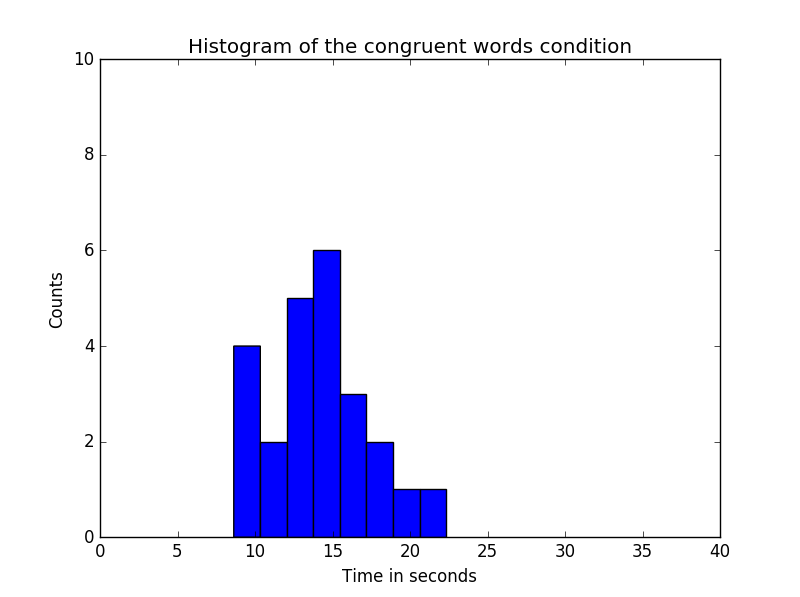
\includegraphics[width=7cm]{figure_1-1.png} }}%
     \qquad
     \subfloat[Histogram of the Incongruent condition]{{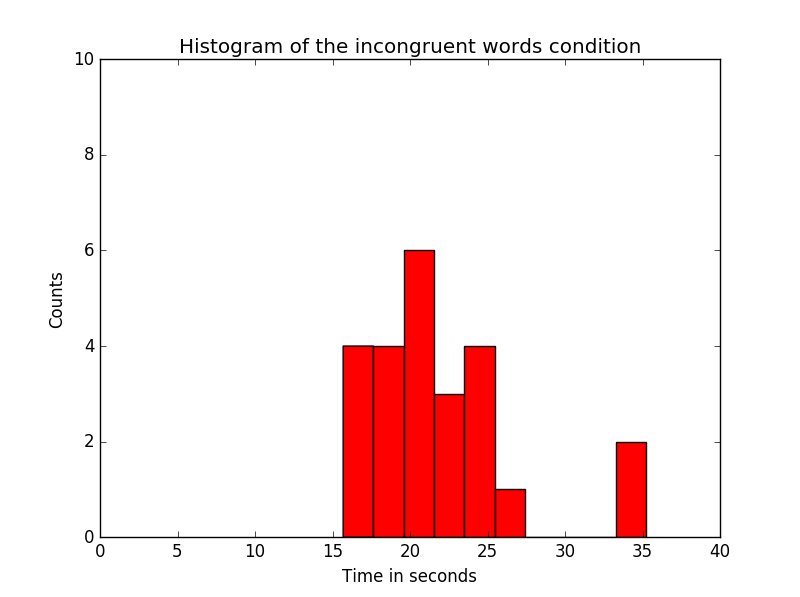
\includegraphics[width=7cm]{figure_2.png} }}%
     \caption{Histograms of the stroop effect data}%
     \label{fig:example}%
 \end{figure}

 \begin{figure}[h]
     \centering
     \subfloat[Comparing both histograms]{{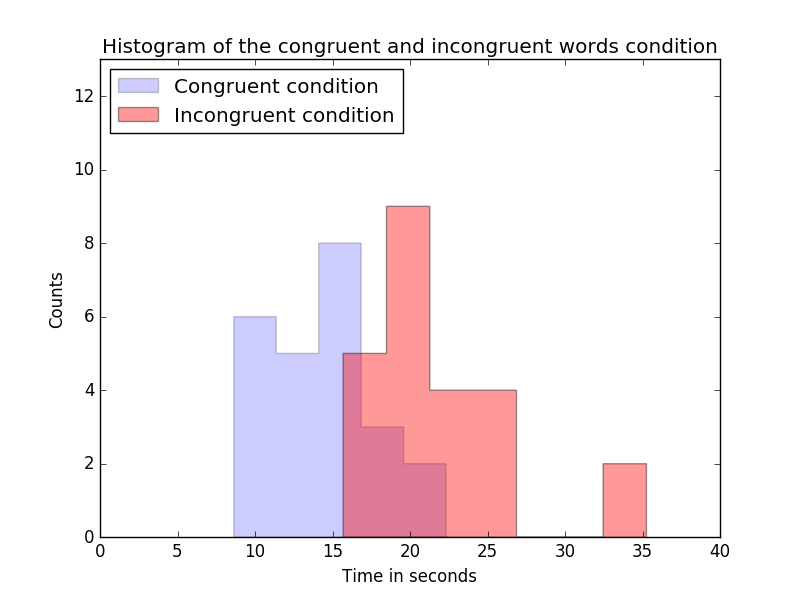
\includegraphics[width=7cm]{figure_3.png} }}%
     \qquad
     \subfloat[Box plot of the dataset]{{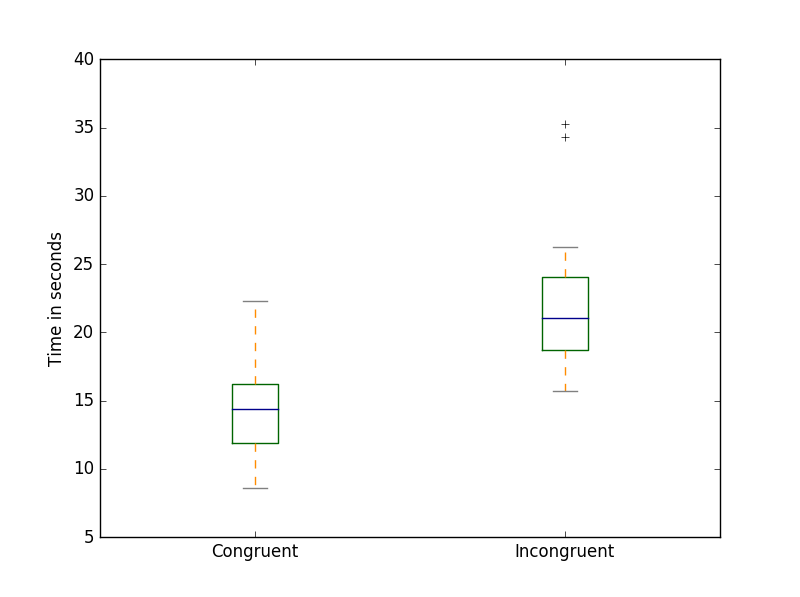
\includegraphics[width=7cm]{figure_4.png} }}%
     \caption{Plots to compare the Congruent and Incongruent data}%
     \label{fig:example}%
 \end{figure}
 
From the histogram plots we can see that the Congruent and Incongruent data peak at different times. We can also clearly see that the mean of the Congruent data is smaller then the Incongruent data. The box plot clearly shows us that their are two outliers in the Incongruent data, which we can also observe in the histogram.  
 
 
\section*{Question 5}
Now, perform the statistical test and report your results. What is your confidence level and your critical statistic value? Do you reject the null hypothesis or fail to reject it? Come to a conclusion in terms of the experiment task. Did the results match up with your expectations?

\subsection*{Solution}

We have already calculated the sample size, means and sample standard deviation of the differences of the data set,  $\bar{x}_{Congruent} = 14.051$, $\bar{x}_{Incongruent} = 22.016$ \& $S = 4.865$ respectively. Using these values now we can perform a t-test.\\

The t-statistic can be calculated as follows:
   \begin{equation}
     t = \frac{\bar{x}_{Congruent} - \bar{x}_{Incongruent}}{\frac{S}{\sqrt{n}}} = -8.02
   \end{equation} 
 
For $\alpha=0.05$ the $t_{critical} = 2.069$ for a two tailed test. Now comparing our results from $t_{critical}$ and the value of $t$ we can conclude that the participants in the Incongruent condition took longer to finish the task.\\

The results of our analysis are as follows:
   \begin{equation}
     t(23) = -8.02, p < .05, two-tailed
   \end{equation} 
Confidence interval on the mean difference; 95\% CI = (-10.02,-5.91). The effect size measures are $d = -1.63$ \& $r^{2} = .73$.\\

From the above analysis and results I reject the null hypothesis. The participants who took the test under the Incongruent conditions took 6 to 10 seconds longer 95\% of the time.

\newline The results did match up to my expectations because when I took the test many times it was impossible for me to finish the task faster under the Incongruent conditions. Also I tried making a guess by looking at the histogram comparison plot. The peaks of the distributions under different conditions are a bit far apart.

\section*{Question 6}
What do you think is responsible for the effects observed? Can you think of an alternative or similar task that would result in a similar effect? Some research about the problem will be helpful for thinking about these two questions!

\subsection*{Solution}
I think that human brain as soon as it processes a text rather then at the color we tent to read it. Its automatic for anyone to just read without any effort but when asked about the color we need to put in some cognitive effort and that delays the response time.

A alternate task which shows the stroop effect is called as the numerical stroop effect. Instead of using the color here different text sizes are used for numbers. the participants are asked to pick out numbers that are numerically larger and not larger just by size.

\newpage
\section*{References}

 \begin{itemize}
 
  \item https://www.verywell.com/what-is-the-stroop-effect-2795832
  
  \item http://pandas.pydata.org/pandas-docs/version/0.18.1/visualization.html

  \item https://imotions.com/blog/the-stroop-effect/
  
  \item http://www.sciencedirect.com/science/article/pii/0028393279900538
  
 \end{itemize}
 
 
 
 
\end{document}
